% 
% This document is available under the Creative Commons Attribution-ShareAlike
% License; additional terms may apply. See
%   * http://creativecommons.org/licenses/by-sa/3.0/
%   * http://creativecommons.org/licenses/by-sa/3.0/legalcode
%
% Created: 2011-08-14 17:43:38+02:00
% Main authors:
%     - Jérôme Pouiller <jezz@sysmic.org>
%

% (cours Tours) patchRT, hyperviseurs

\tikzstyle{main}     = [node distance=1cm, transform shape, inner sep=0pt, outer sep=0pt, rounded corners=2mm, text centered, minimum height=0.9cm]
\tikzstyle{cred}     = [fill=red!20!white,     draw=red!50!black,     rounded corners=2mm]
\tikzstyle{cblue}    = [fill=blue!20!white,    draw=blue!50!black,    rounded corners=2mm]
\tikzstyle{cgreen}   = [fill=green!20!white,   draw=green!50!black,   rounded corners=2mm]
\tikzstyle{corange}  = [fill=orange!20!white,  draw=orange!50!black,  rounded corners=2mm]
\tikzstyle{cyellow}  = [fill=yellow!20!white,  draw=yellow!50!black,  rounded corners=2mm]
\tikzstyle{ccyan}    = [fill=cyan!20!white,    draw=cyan!50!black,    rounded corners=2mm]
\tikzstyle{cbrown}   = [fill=brown!20!white,   draw=brown!50!black,   rounded corners=2mm]
\tikzstyle{cpurple}  = [fill=purple!20!white,  draw=purple!50!black,  rounded corners=2mm]
\tikzstyle{size1}=[main, minimum width=1.9cm, text width=1.8cm]
\tikzstyle{size2}=[main, minimum width=3.9cm, text width=3.8cm]
\tikzstyle{size3}=[main, minimum width=5.9cm, text width=5.8cm]
\tikzstyle{size4}=[main, minimum width=7.9cm, text width=7.8cm]

\part{Architectures des OS temps réels}

\section{Problématique des OS RT} %(45min)

\begin{frame}{Limites des système classiques}
  Les systèmes classiques s'appuient sur un système d'exploitation en général mal adapté pour le temps réel:
  \begin{itemize}
  \item Politique d'ordonnancement visant à équiliber équitablement le temps alloué à chaque tâche
  \item Mécanismes d'accès aux ressources partagées et de synchronisation comportent des incertitudes temporelles
  \item Gestion des interruptions non-optimisées
  \item La gestion de la mémoire virtuelle, des caches engendrent des fluctuation temporelles
  \item La gestion des temporisateurs qui servent à la manipulation des temps pas assez fin
  \end{itemize} 
\end{frame}

\begin{frame}{Contexte}
  Garantie qu'une action est éxecutée en moins d'un temps donné.

  Implique:
  \begin{itemize}
    \item Une garantie de qualité (0 bug)
    \item Souvent des processus garantissant la qualité dans les différentes phases: conception, développement, validation
    \item Une connaissances importante de l'environnement extérieur (fréquence maximum des interruption, etc...)
  \end{itemize}
  $\to$ On se limitera à l'architecture logicielle
\end{frame}

\begin{frame}{Contexte}
  Ordonnancement statique:
  \begin{itemize}
    \item Charge des taches temps réelles $\ll 100\%$
    \item[$\to$] Ordonnancement avec des priorités statiques suffisante
    \item[$\to$] Problématique des algorithmes d'ordonnancement à priorité dynamique (EDF, LST, etc...) secondaire
  \end{itemize}
\end{frame}

% En d'autre termes:
\begin{frame}{Contexte}
$$
R_i = C_i + \sum_{j \in hp(i)} \left\lceil\frac{R_i}{T_j}\right\rceil C_j
$$
Pour les allergiques: le temps de réponse d'une tâche est égal à la somme du
temps d'exécution de la tache et de toutes les tâche de priorité supérieure
qui s'exécutent en même temps.\\[1.5ex]
Objectif: Rendre cette formule assez simple pour être prédictible.\\[1.5ex]
Pas si simple:
  \begin{itemize}
    \item Interruptions
    \item Changement de contexte
    \item Sections critiques (ordonnanceur désactivé)
    \item Caches, Swap
  \end{itemize}
\end{frame}

% Schema des temps de réponses
% La principale chose que nous allons combattre, sera le temps de réponse aux
% évènements. Le temps de réponse peut-être très aléatoire
% Si on avait un temps de réponse null (ou au moins constant). Alors, il
% deviendrait simple de calculer les temps de réponse maximum de nos taches
\begin{frame}{Latence aux évènements}
  \begin{itemize}
    \item Coeur du problème
    \item Si la latence était  nul (ou au moins constante), on calculerait
      simplement le temps de réponses de nos tâches.
  \end{itemize}

\begin{preview}  
  \begin{center}
   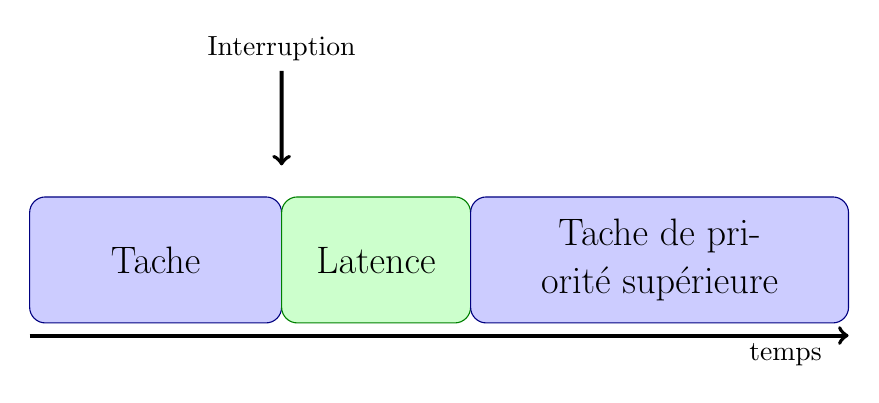
\begin{tikzpicture}[scale=0.8]
     \tikzstyle{msize}=[main, minimum height=2cm, font=\LARGE]
     \draw
       node[anchor=south]                at (2, 3) {Interruption}
       edge[->, line width=0.5mm]  (2, 1.5)
       node[msize, cblue,  minimum width=4cm, text width=4cm] at (  0, 0) {Tache}
       node[msize, cgreen, minimum width=3cm, text width=3cm] at (3.5, 0) {Latence}
       node[msize, cblue,  minimum width=6cm, text width=6cm] at (  8, 0) {Tache de priorité supérieure}
       (-2, -1.2) edge[->, line width=0.5mm]  (11, -1.2)
       node at (10, -1.5) {temps};
   \end{tikzpicture}
  \end{center}
\end{preview}
\end{frame}

\begin{frame}{Latence aux évènements}{Exemple concret}
\begin{itemize}
 \item On paramètre un timer à 50Hz
 \item On mesure le temps effectif de chaque période
\end{itemize}
\end{frame}

% Exemple concret
% Expliquer que l'on paramètre un timer à 50Hz
% On mesure les période effectives
% Le temps de réponse est ici très aléatoire et dépend fortement de la charge de la machine
% Schema des temps de réponses
\begin{frame}{Latence aux évènements}{Système classique}
  \begin{center}
    \pgfimage[width=10cm]{pics/latency_2}
  \end{center}
\end{frame}

% Le temps de réponse ici est beaucoup mieux borné
% Schema des temps de réponses
\begin{frame}{Latence aux évènements}{Système temps réels}
  \begin{center}
    \pgfimage[width=10cm]{pics/latency_1}
  \end{center}
\end{frame}
%     -> Taches RT << 100\%
%     ->  --> Algorithme d'ordonnancement secondaire (RM vs EDF)
%     -> Rendre cette formule assez simple pour être prédictible
%     %-> CAD limiter les effets des tache apériodique de priorité supérieure:
%        Interruptions, cache miss, changement de contexte, etc...
%     -> Présenter les diagramme normal va RT

\section{Systèmes Symétrique et asymétriques}

\begin{frame}{Systèmes symétriques}
\end{frame} 

\begin{frame}{Systèmes asymétriques}
\end{frame} 

\section{Low-latency}

\begin{frame}{Noyau low latency}{Problème du noyau normal} % 10min
 Un seul contexte noyau pour tout le monde
 \begin{itemize}
  \item Pas possible de préempter le système
  \item Personne ne peut prendre la main lorsqu'un processus est dans un syscall
  \item Équivalent d'une ressource partagée par tout les processus
  \item Possible de créer une gigantesque inversion de priorité
 \end{itemize}
\end{frame}

\begin{frame}{Noyau low latency}{Implémentation} % 10min
 \begin{itemize}
  \item Difficile de gérer les différents contextes noyau
  \item[$\to$] Noyau réentrant (= thread-safe)
  \item Gestion des interruption assez complexe
  \item Overhead assez important
 \end{itemize}
\end{frame}
%         -> Explique le problème des contexte noyaux
%         -> Définition de "Réentrant" (thread-safe)

\begin{frame}{Noyau low latency}{Résultats} % 5min
 \begin{itemize}
   \item Patch low-latency mergé dans le mainstream avec le noyau 2.6 (\texttt{CONFIG\_PREEMPT})
   \item Latences maximum de l'ordre de 300µs (chiffres de l'époque)
 \end{itemize}
\end{frame}
%      -> Patch low-latency, mergé dans le mainstream avec le noyau 2.6 (CONFIG\_PREEMPT)
%      -> A l'époque, on obtenait des latence max de l'ordre de 300µs

\section{Hyperviseurs} % (30min)

\begin{frame}{Hyperviseur}
  \begin{itemize}
    \item Noyau low latency encore problèmatique pour les interruptions
    \item Beaucoup d'interruptions $\to$ latence
    \item Hyperviseur
  \end{itemize}
\end{frame}
%      -> Utilisation d'un hyperviseur
%      -> Shéma RTLinux et ADEOS

% \begin{frame}{Temps réel}{Micro Kernel}
%   \includegraphics[height=6cm]{pics/RT-microKernel}
% \end{frame}
% 
% \begin{frame}{Temps réel}{Nano Kernel}
%   \includegraphics[height=6cm]{pics/RT-nanoKernel}
% \end{frame}
\begin{frame}{Temps réel}{Nano Kernel}
  \begin{center}
    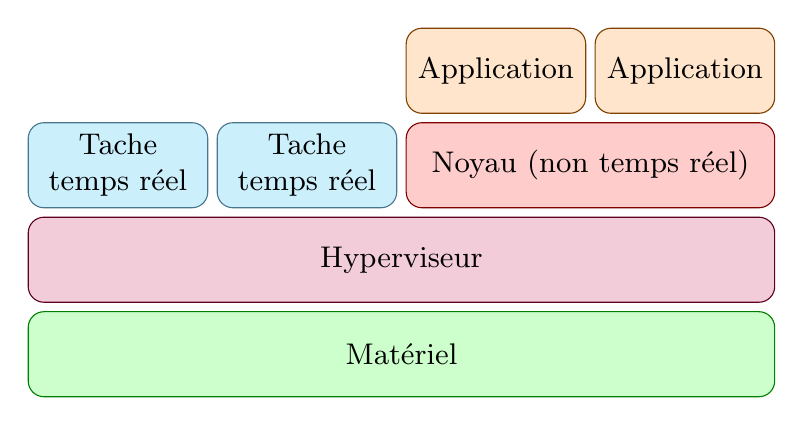
\begin{tikzpicture}[scale=1.2]
      \draw[font=\small]
        node[size1, ccyan]   at (1, 2) {Tache temps réel}
        node[size1, ccyan]   at (3, 2) {Tache temps réel}
        node[size1, corange] at (5, 3) {Application}
        node[size1, corange] at (7, 3) {Application}
        node[size2, cred]    at (6, 2) {Noyau (non temps réel)}
        node[size4, cpurple] at (4, 1) {Hyperviseur}
        node[size4, cgreen]  at (4, 0) {Matériel};
    \end{tikzpicture}
  \end{center}
\end{frame}

\begin{frame}[fagile]{Hyperviseur}
  \begin{itemize}
   \item Possibilité de préempter le noyau sans patch low-latency
   \item Possibilité de differer les interruptions
   \item Possibilité d'ignorer les interruptions dans les sections temps réelles
   \item Performances excellentes (< 20µs)
   \item Technique non spécifique à Linux
   \item Peu de code en mode temps réelles
   \item[$\to$] Certifiable

   \item Fonctionne au dessus du noyau
   \item Comportement des interruptions à modifier
   \item Communication entre les tâches temps réelles et le reste
   \item[$\to$] Nécessite de patcher le noyau
   
   \item RTLinux, RTAI et Adeos (\texttt{http://download.gna.org/adeos/patches/}, \texttt{git://git.xenomai.org/ipipe-gch.git}) (Xenomai)
  \end{itemize}
\end{frame}

\begin{frame}{Hyperviseur}{Adeos}
  \begin{itemize}
    \item Fork de RTAI
    \item API utilisateur assurée par Xenomai
    \begin{itemize}
      \item Skins 
      \item[$\to$] Possibilité de faire fonctionner une application développée pour vxWorks
% Parler de vxWorks: Référence dans le domaine des OS RT Posix, OS des sondes Martiennes
      \item Skin native consistante
      \item Beaucoup mieux que Posix (de plus, il existe une skin Posix)
      \item \texttt{www.xenomai.org/documentation/xenomai-head/html/api}
    \end{itemize}
  \end{itemize}
\end{frame}
%      -> API utilisateur assurée par Xenomai
%         -> Skin, possibilité de faire fonctionner une application faite pour vxWorks
%         -> Skin native consistante
%         -> Beaucoup mieux que Posix (de plus, il existe une skin Posix)

% TP Interuptions avec Xenomai
% Mettre en place l'interruption RTC (8) voir Doucmentation/rtc.txt
\section{RT-préempt} % (30min)

\begin{frame}{RT-preempt} % (15min)
  Gestion des interruption dans des threads
%     -> Rappeller vous de nos spin_lock
  \begin{itemize}
    \item Permet de préempter les interruptions
    \item[$\to$] Moins de latence des taches
    \item Permet d'ordonnancer les interruption
    \item[$\to$] Permet de se passer de la désactivation des interruptions
    \item[$\to$] Permet de remplacer les spin lock par des mutex
    \item[$\to$] Moins de latence des interruptions
  \end{itemize}
\end{frame}

\begin{frame}{RT-preempt} 
  \begin{center}
    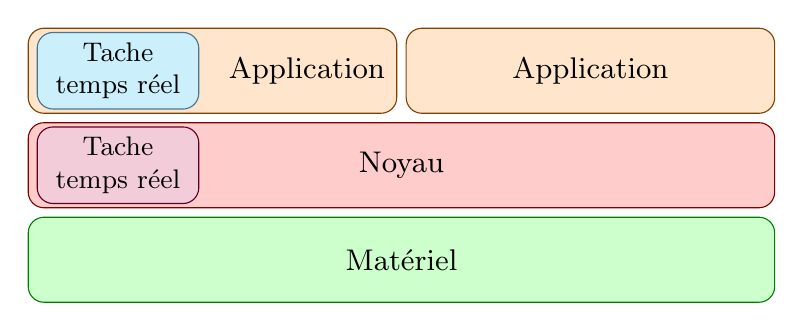
\begin{tikzpicture}[scale=1.2]
      \draw[font=\small]
        node[size2, corange]    at (6, 2) {Application}
        node[size2, corange]    at (2, 2) { } 
        node[size1]             at (3, 2) {Application}
        node[size1, ccyan, scale=0.9] at (1, 2) {Tache temps réel}
        node[size4, cred]       at (4, 1) { } 
        node[size3]             at (4, 1) {Noyau}
        node[size1, cpurple, scale=0.9] at (1, 1) {Tache temps réel}
        node[size4, cgreen]     at (4, 0) {Matériel};
    \end{tikzpicture}
  \end{center}
\end{frame}

\begin{frame}{RT-preempt}
 \begin{itemize}
  \item Patch RT (Patchs: \texttt{http://www.kernel.org/pub/linux/kernel/projects/rt/}, Git: \texttt{git://git.kernel.org/pub/scm/linux/kernel/git/rostedt/linux-2.6-rt.git})
  \item Implémentation assez complexe
  \item[$\to$] Non portable
  \item Performance très bonnes (~20µs)
 \end{itemize}
\end{frame}
%     -> Gère les interruption dans des thread
%     -> /!\ Pas portable partout
%     -> Implémentation assez tordue (c'est un cinglé qui a fait ca).
%     -> PatchRT
